
% file: unique_paths.tex

\problemsection{Unique Paths}
\label{problem:unique_paths}
\marginnote{A classic dynamic programming problem that demonstrates how to build complex solutions from simpler subproblems.}

\section*{Problem Statement}
Given a \(m \times n\) grid, a robot starts at the top-left corner (marked 'Start') and aims to reach the bottom-right corner (marked 'Finish'). The robot can only move either down or right at each step. Calculate the total number of unique paths possible.

\begin{figure}[h]
    \centering
    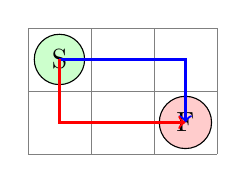
\begin{tikzpicture}[scale=0.8]
        \draw[step=1cm,gray,very thin] (0,0) grid (3,2);
        \node[draw,circle,fill=green!20] at (0.5,1.5) {S};
        \node[draw,circle,fill=red!20] at (2.5,0.5) {F};
        \draw[->,blue,thick] (0.5,1.5) -- (2.5,1.5) -- (2.5,0.5);
        \draw[->,red,thick] (0.5,1.5) -- (0.5,0.5) -- (2.5,0.5);
    \end{tikzpicture}
    \caption{Example of a 3×2 grid showing two possible paths}
    \label{fig:unique_paths}
\end{figure}

\textbf{Examples:}
\begin{verbatim}
Input: m = 3, n = 2
Output: 3
Explanation: From top-left corner, there are three ways:
1. Right → Right → Down
2. Right → Down → Right
3. Down → Right → Right

Input: m = 3, n = 7
Output: 28
\end{verbatim}

\section*{Solution Approaches}

\subsection*{1. Dynamic Programming (Optimal)}
\begin{itemize}
    \item \textbf{Time:} O(m×n)
    \item \textbf{Space:} O(m×n) or O(n) with optimization
    \item \textbf{Idea:} Each cell's paths = paths from above + paths from left
\end{itemize}

\subsection*{2. Combinatorics}
\begin{itemize}
    \item \textbf{Time:} O(min(m,n))
    \item \textbf{Space:} O(1)
    \item \textbf{Formula:} C(m+n-2, m-1) or C(m+n-2, n-1)
\end{itemize}

\section*{Optimal Implementation}
\begin{fullwidth}
\begin{lstlisting}[language=Python]
from typing import List

class Solution:
    def uniquePaths(self, m: int, n: int) -> int:
        # Optimize space by using 1D DP array
        dp = [1] * n
        
        for i in range(1, m):
            for j in range(1, n):
                dp[j] += dp[j-1]
        
        return dp[-1]

    def uniquePathsCombinatorics(self, m: int, n: int) -> int:
        # Alternative combinatorics solution
        def nCr(n: int, r: int) -> int:
            r = min(r, n-r)  # Optimize by using smaller r
            numerator = denominator = 1
            for i in range(r):
                numerator *= (n - i)
                denominator *= (i + 1)
            return numerator // denominator
            
        return nCr(m + n - 2, min(m - 1, n - 1))

# Test cases
def test_unique_paths():
    solution = Solution()
    
    # Basic cases
    assert solution.uniquePaths(3, 2) == 3
    assert solution.uniquePaths(3, 7) == 28
    
    # Edge cases
    assert solution.uniquePaths(1, 1) == 1
    assert solution.uniquePaths(1, 5) == 1
    assert solution.uniquePaths(5, 1) == 1
\end{lstlisting}
\end{fullwidth}

\section*{Implementation Details}
\begin{itemize}
    \item \textbf{Space Optimization:} Using 1D DP array instead of 2D
    \item \textbf{Base Cases:} First row and column initialized to 1
    \item \textbf{DP Formula:} dp[j] += dp[j-1]
    \item \textbf{Alternative:} Combinatorics solution included
\end{itemize}

\section*{Common Pitfalls}
\begin{itemize}
    \item Forgetting to initialize first row/column
    \item Using unnecessary 2D array
    \item Integer overflow in combinatorics approach
    \item Not handling edge cases (m=1 or n=1)
\end{itemize}

\section*{Interview Tips}
\begin{itemize}
    \item Start with the DP solution - it's more intuitive
    \item Mention space optimization possibility
    \item Discuss the combinatorics approach as optimization
    \item Consider follow-up questions:
        \begin{itemize}
            \item What if there are obstacles?
            \item What if certain cells are blocked?
            \item What if diagonal moves are allowed?
        \end{itemize}
\end{itemize}

\section*{Related Problems}
\begin{itemize}
    \item Unique Paths II (with obstacles)
    \item Minimum Path Sum
    \item Robot Room Cleaner
    \item Cherry Pickup
\end{itemize}

\printindex